\section{Results}
\label{sec:results}

Figures~\ref{fig:fig1}--\ref{fig:fig3} summarize the simulation study. We
organize the Results section around the visual message of each figure: first,
whether perturbed steady states contain enough information to recover a signed
nonlinear network; second, how recovery depends on sample budget and
perturbation design; and third, how PSS-Net behaves relative to external
methods, graph topology, and measurement scale.

\subsection{Finding 1: steady-state endpoints recover signed nonlinear network
structure}
\label{sec:res:foundation}

\paragraph{The endpoint response, not the transient path, is the object of
inference.}
Figure~\ref{fig:fig1}a contrasts additive and multiplicative gLV transients that
converge to the measured perturbed equilibria. The figure highlights the
operational input to PSS-Net: the post-perturbation steady-state pair
$(\tilde{\xv}^{(k)},\uv^{(k)})$, rather than numerical derivatives along the
trajectory. Figure~\ref{fig:fig1}b then shows that nonlinear steady-state
signatures are separable when the signal-to-noise ratio is sufficient, whereas
the same signatures collapse toward the linear/additive alternatives under
larger measurement noise.

\paragraph{Node-wise \adsiht{} gives stable directed-support recovery across
network sizes.}
In Fig.~\ref{fig:fig1}c, edge-recovery performance remains near MCC 0.9 at the
largest displayed scaled budget across $p=8$, 30, and 100. The endpoint MCC for
\adsiht{} was $0.901\pm0.066$ and $0.898\pm0.066$ for $p=8$ under linear and
nonlinear truth, $0.904\pm0.023$ and $0.902\pm0.029$ for $p=30$, and
$0.908\pm0.012$ and $0.909\pm0.012$ for $p=100$. Group lasso also improved
with budget, but its endpoint MCC ranged more widely, from $0.614\pm0.092$ to
$0.921\pm0.074$ in the same endpoint comparisons.

\paragraph{Recovered edges correspond to signed functional effects, not only
edge scores.}
Figures~\ref{fig:fig1}d--f connect the recovered support to fitted regulatory
functions and the inferred directed graph. In the function-shape recovery
summary, all 16 true cross-node effects and all 10 self-effects were selected,
whereas null cross-node pairs had mean selected rate $0.034\pm0.036$ across 74
pairs. The mean curve RMSE was 0.004 for true cross-node effects, 0.002 for
self-effects, and 0.001 for null cross-node pairs.

\paragraph{Support recovery is robust to moderate basis mismatch, while
function-shape recovery is basis-dependent.}
Figure~\ref{fig:fig1}g separates two outputs. Across quadratic, Monod-type, and
sinusoidal truth, support MCC stayed between 0.788 and 0.916 over the five
fitted libraries. Edge-function NRMSE varied more: for quadratic truth it was
$0.072\pm0.024$ with the quadratic library and $0.211\pm0.080$ with the cubic
library; for Monod truth it was $0.104\pm0.024$ with the Monod library and
$0.354\pm0.062$ with the cubic library; and for sinusoidal truth it was
$0.106\pm0.013$ with the quadratic library and $0.264\pm0.056$ with the Monod
library.

\begin{figure}[t]
  \centering
  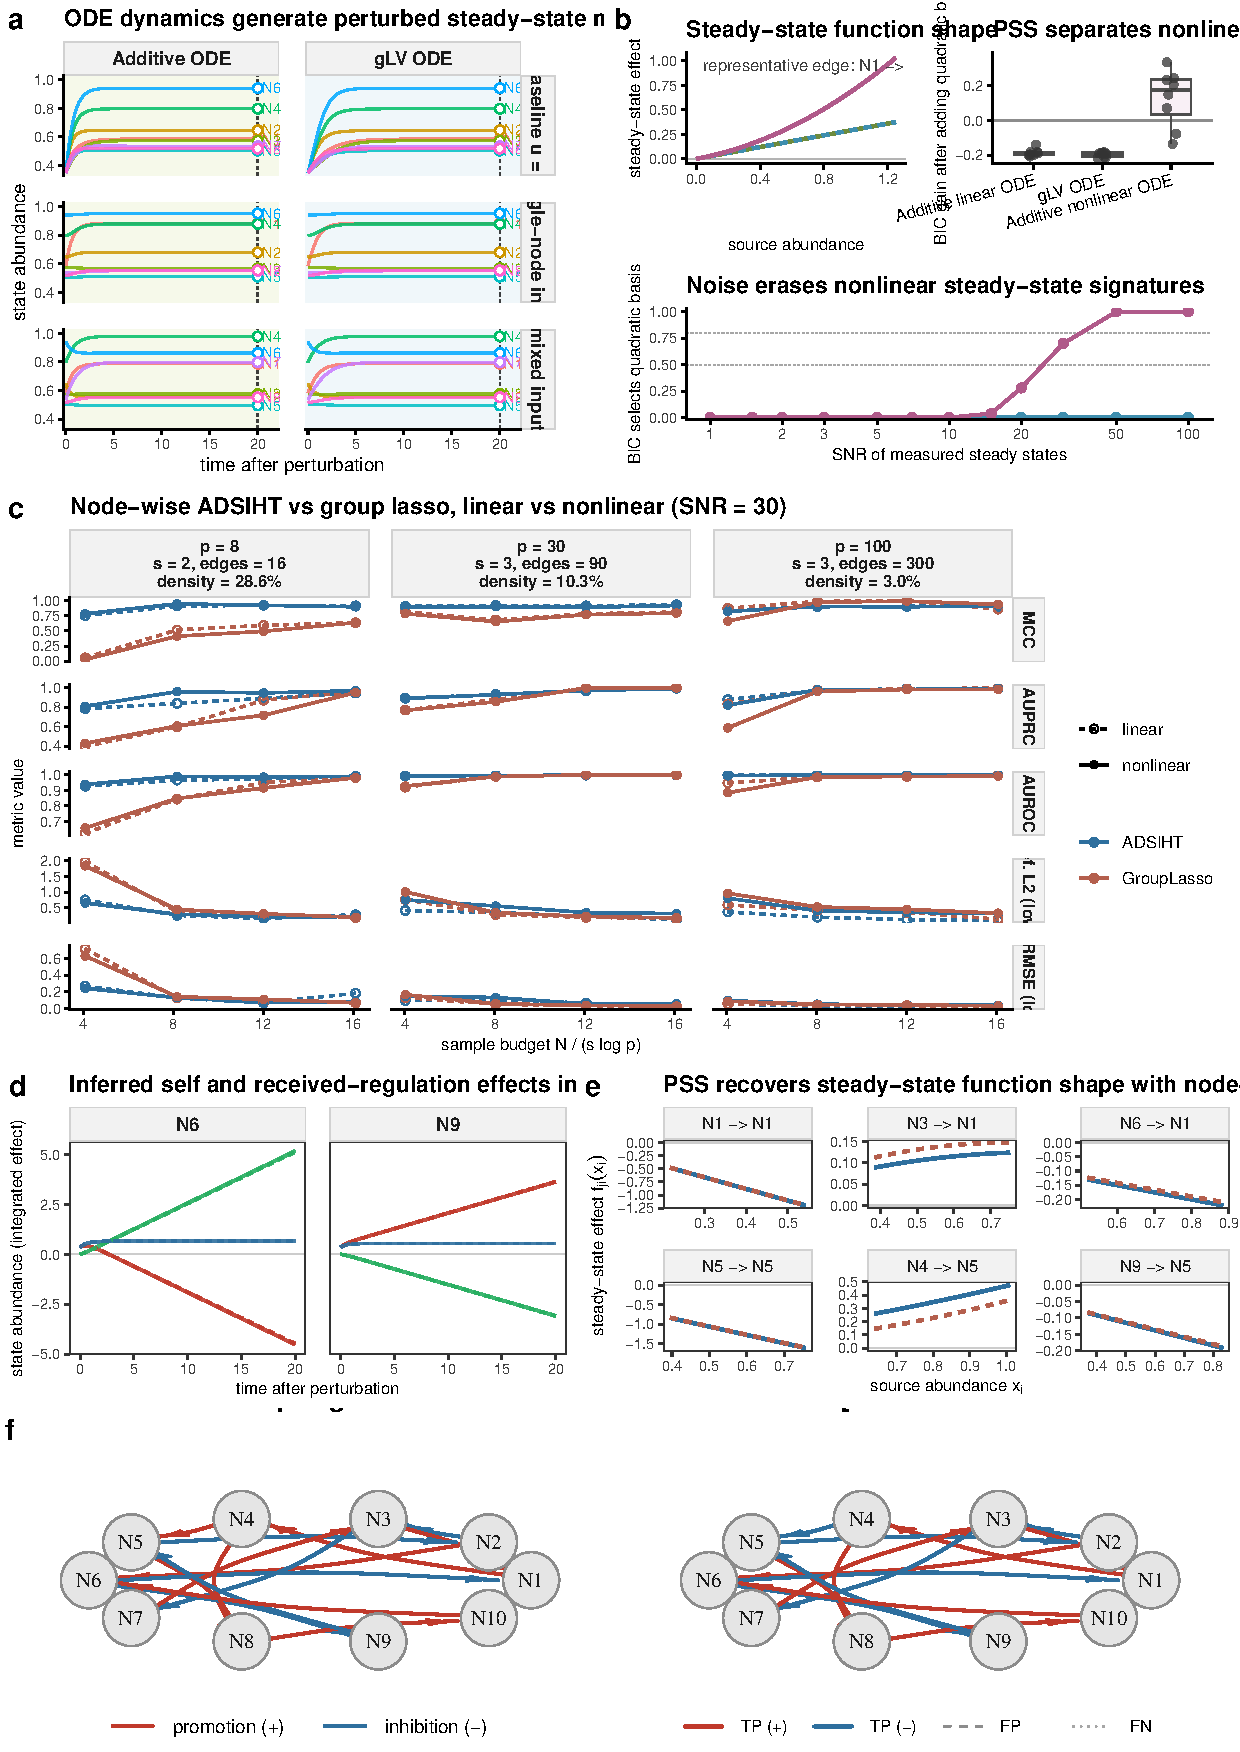
\includegraphics[width=\linewidth]{Fig1.pdf}
  \caption{\textbf{Perturbed steady states identify the directed network.}
  (a) Additive versus multiplicative gLV dynamics converging to the same
  measured steady state. (b) Function-shape identifiability across
  signal-to-noise ratio. (c) Node-wise \adsiht{} versus group lasso edge
  recovery across problem sizes. (d) Self and received cross-node effects
  integrating to the trajectory, true versus inferred. (e) Per-source
  edge-function recovery. (f) True versus inferred directed coupling network.
  (g) Library misspecification: support MCC versus edge-function NRMSE. Points
  show individual replicates from 30 simulations; summaries show mean $\pm$
  s.d.}
  \label{fig:fig1}
\end{figure}

\subsection{Finding 2: sparse sample budget governs recovery, and design gains
are regime-dependent}
\label{sec:res:design}

\paragraph{The recovery curves align with the sparse budget scale.}
Figure~\ref{fig:fig2}a plots MCC against $N/(s\log p)$ for $p=8$, 50, and 100.
At $N/(s\log p)\approx1$, mean MCC was 0.038, 0.039, and 0.027 for these three
sizes. Around $N/(s\log p)\approx8$, the corresponding values were 0.595,
0.746, and 0.751. At the largest displayed budgets, they reached 0.909, 0.921,
and 0.907.

\paragraph{Designed perturbations help most before random designs saturate.}
Figure~\ref{fig:fig2}b illustrates the design choices, and
Fig.~\ref{fig:fig2}c shows that the MCC gain over random depends on both the
truth regime and the budget. In the nonlinear benchmark, random perturbations
had mean MCC 0.049 at $N=12$ and 0.509 at $N=60$, whereas maximin reached 0.123
and 0.654. Oracle D-optimal design, available from $N=20$, reached MCC 0.220,
0.417, 0.508, and 0.650 at $N=20,30,40,60$. In the strong-nonlinear benchmark,
random perturbations had MCC 0.097 at $N=12$ and 0.521 at $N=60$; maximin gave
0.136 and 0.664; and oracle D-optimal gave 0.376, 0.451, 0.578, and 0.640 at
$N=20,30,40,60$.

\paragraph{Budget-to-target plots show when design changes the experimental
requirement.}
Figure~\ref{fig:fig2}d converts recovery curves into the budget required to
reach fixed MCC targets. The visual pattern is consistent with
Fig.~\ref{fig:fig2}c: structured designs change the required budget most in
the nonlinear regimes, while differences are smaller once the curves approach
the high-MCC plateau.

\paragraph{Pilot-informed D-optimal design is competitive at larger total
budgets.}
Figure~\ref{fig:fig2}e replaces the oracle response map with a pilot-estimated
map. At total budget $N_{\mathrm{total}}=60$, pilot-informed D-optimal design
had MCC $0.674\pm0.128$, $0.648\pm0.136$, and $0.630\pm0.122$ for pilot sizes
8, 12, and 16. The corresponding random-design MCC values were
$0.534\pm0.094$, $0.538\pm0.098$, and $0.493\pm0.119$. At
$N_{\mathrm{total}}=20$, pilot-informed D-optimal MCC remained between 0.190
and 0.219.

\begin{figure}[t]
  \centering
  
\includegraphics[width=\linewidth]{Fig2.pdf}
  \caption{\textbf{Sample complexity and active perturbation design.}
  (a) Edge MCC versus the rescaled budget $N/(s\log p)$. (b) Input-space
  schematic of the random, maximin, oracle, and pilot-estimated D-optimal
  designs. (c) Mean MCC gain over random across regime and budget.
  (d) Budget required to reach fixed MCC targets. (e) Oracle and
  pilot-informed D-optimal design results. Summaries are computed across 30
  independent simulations.}
  \label{fig:fig2}
\end{figure}

\subsection{Finding 3: PSS-Net matches response-matrix recovery and exposes
model-level limits}
\label{sec:res:benchmark}

\paragraph{The capability matrix distinguishes what each method can return.}
Figure~\ref{fig:fig3}a positions PSS-Net with respect to the benchmarked
alternatives. PSS-Net returns directed, signed, nonlinear, perturbation-based
network structure and fitted edge functions. MRA/aiMeRA provides a directed
signed response matrix, but not absolute-scale edge functions; association
methods provide neither directionality nor perturbation-specific functional
effects.

\paragraph{At the representative benchmark budget, PSS-Net and aiMeRA have
matched edge-selection scores.}
At $N=171$ ($N/(s\log p)=25.138$) in Fig.~\ref{fig:fig3}b, PSS-Net and aiMeRA
both achieved MCC 1.000 and AUPRC 1.000 under linear truth. Under strong
nonlinear truth, PSS-Net had MCC $0.965\pm0.017$ and AUPRC $0.990\pm0.010$,
while aiMeRA had MCC $0.964\pm0.016$ and AUPRC $0.987\pm0.014$. Lasso reached
MCC $0.629\pm0.089$ under strong nonlinear truth; PySINDy-STLSQ reached
$0.454\pm0.044$; and correlation and partial correlation were below 0.27 MCC.

\paragraph{Joint estimation changes recovery most on scale-free graphs.}
Figure~\ref{fig:fig3}c displays the two topology classes, and
Fig.~\ref{fig:fig3}d compares node-wise and joint PSS-Net. On scale-free
graphs, joint PSS-Net increased mean MCC from 0.080 to 0.110 at $N=16$, 0.202
to 0.259 at $N=24$, 0.355 to 0.408 at $N=32$, and 0.484 to 0.520 at $N=40$.
The out-degree rank correlation also increased from 0.144 to 0.188, 0.295 to
0.367, 0.442 to 0.557, and 0.529 to 0.642. On Erd\H{o}s--R\'enyi graphs, MCC
differences were smaller: 0.094 versus 0.112 at $N=16$, 0.254 versus 0.305 at
$N=24$, 0.441 versus 0.440 at $N=32$, and 0.590 versus 0.603 at $N=40$.

\paragraph{Measurement scale is a major limitation.}
In Fig.~\ref{fig:fig3}e, absolute-abundance inputs gave MCC
$0.890\pm0.052$. Relative abundance reduced MCC to $0.520\pm0.124$, and
centered log-ratio inputs gave $0.317\pm0.129$. In the current simulation, the
relative-abundance input multiplied by a noisy total had MCC
$-0.047\pm0.134$, with lower precision than the relative-abundance input.

\begin{figure}[t]
  \centering
  
\includegraphics[width=\linewidth]{Fig3.pdf}
  \caption{\textbf{External benchmarks, topology dependence, and compositional
  limits.} (a) Method capability matrix. (b) Edge-recovery benchmark against
  MRA/aiMeRA, sparse regression, PySINDy-STLSQ, and association baselines.
  (c) Scale-free versus Erd\H{o}s--R\'enyi topology schematic. (d) Node-wise
  versus joint PSS-Net recovery on the two topologies. (e) Recovery across
  absolute, relative, centered-log-ratio, and total-multiplied relative
  measurement scales. Summaries are computed across 30 independent simulations.}
  \label{fig:fig3}
\end{figure}
